% =========================================================
% Chapter 6 - Hiện thực, kiểm thử và đánh giá hệ thống
% Project: AITasker
%
% Yêu cầu trong main.tex:
% \usepackage{graphicx}
% \usepackage{float}
% \usepackage{longtable}
% \usepackage{array}
% \usepackage{booktabs}
% \usepackage{enumitem}
% \graphicspath{{figures/}}
%
% Tên hình được sử dụng đúng theo thư mục figures:
%   login.png
%   register.png
%   dashboard.png
%   projects.png
%   contracts.png
%   assistant.png
%   payment.png
%   analytics.png
%   statistics_dashboard.png
%   aiservices.png
% =========================================================

\chapter{Hiện thực, kiểm thử và đánh giá hệ thống}
\label{chap:implementation-testing}

\section{Giới thiệu}
\label{sec:chapter6-introduction}

Chương này trình bày kết quả hiện thực giao diện của hệ thống AITasker, mô tả các màn hình chức năng chính và đánh giá mức độ đáp ứng yêu cầu đã đặc tả. Các hình ảnh được lấy trực tiếp từ phiên bản hệ thống đang chạy trên môi trường phát triển, qua đó chứng minh sự liên kết giữa thiết kế, mã nguồn và sản phẩm thực tế.

Nội dung chương gồm ba phần chính:

\begin{itemize}
    \item Giới thiệu các giao diện chức năng đã hiện thực.
    \item Trình bày các kịch bản kiểm thử chức năng và tích hợp.
    \item Đánh giá kết quả, ưu điểm, hạn chế và mức độ hoàn thành hệ thống.
\end{itemize}

\section{Môi trường hiện thực và kiểm thử}
\label{sec:implementation-environment}

\begin{table}[H]
    \centering
    \caption{Môi trường hiện thực và kiểm thử}
    \label{tab:implementation-environment}
    \begin{tabular}{|p{4.4cm}|p{9.0cm}|}
        \hline
        \textbf{Thành phần} & \textbf{Công nghệ/Cấu hình} \\ \hline
        Hệ điều hành & Windows 10/11 \\ \hline
        Frontend & ReactJS, Vite, HTML, CSS, JavaScript \\ \hline
        Backend & Python 3.12, FastAPI, Uvicorn \\ \hline
        Cơ sở dữ liệu & PostgreSQL \\ \hline
        ORM và migration & SQLAlchemy, Alembic \\ \hline
        Xác thực & JWT, BCrypt \\ \hline
        Trình duyệt kiểm thử & Google Chrome, Microsoft Edge \\ \hline
        Công cụ kiểm thử API & Swagger UI \\ \hline
        Môi trường phát triển & Visual Studio Code \\ \hline
    \end{tabular}
\end{table}

\section{Giao diện xác thực người dùng}
\label{sec:authentication-interface}

\subsection{Giao diện đăng nhập}

Giao diện đăng nhập cho phép người dùng nhập tài khoản hoặc email và mật khẩu để truy cập hệ thống. Sau khi thông tin được gửi, backend xác minh tài khoản, kiểm tra mật khẩu đã băm bằng BCrypt, trạng thái tài khoản và cấp JWT nếu xác thực thành công.

\begin{figure}[H]
    \centering
    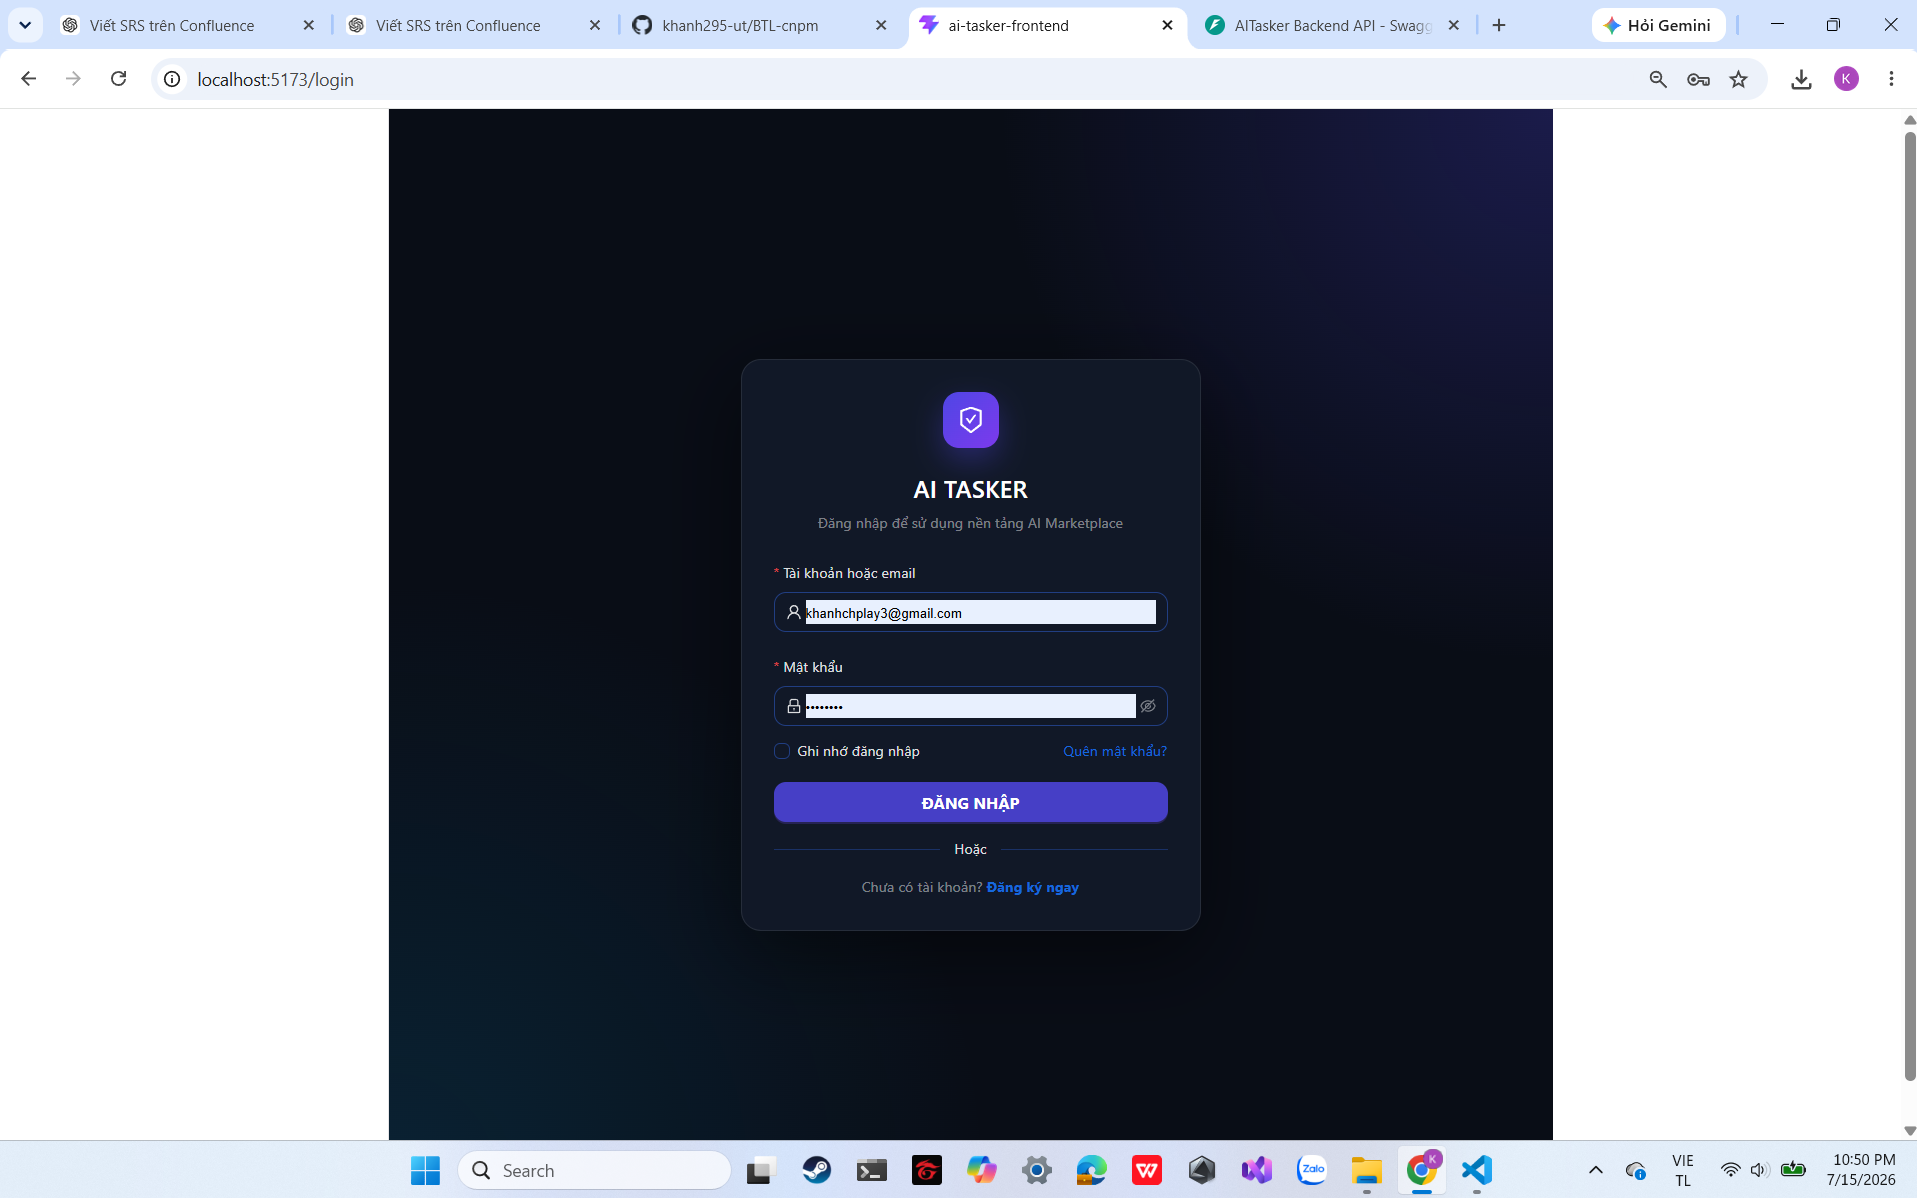
\includegraphics[width=0.78\textwidth]{login.png}
    \caption{Giao diện đăng nhập hệ thống AITasker}
    \label{fig:ui-login}
\end{figure}

Giao diện hỗ trợ các thành phần:

\begin{itemize}
    \item Trường tài khoản hoặc email.
    \item Trường mật khẩu và chức năng hiển thị/ẩn mật khẩu.
    \item Tùy chọn ghi nhớ đăng nhập.
    \item Liên kết quên mật khẩu.
    \item Liên kết chuyển sang trang đăng ký.
\end{itemize}

\subsection{Giao diện đăng ký}

Giao diện đăng ký cho phép người dùng mới tạo tài khoản doanh nghiệp hoặc chuyên gia AI. Hệ thống kiểm tra các trường bắt buộc, định dạng email, độ mạnh mật khẩu và xác nhận mật khẩu trước khi tạo tài khoản.

\begin{figure}[H]
    \centering
    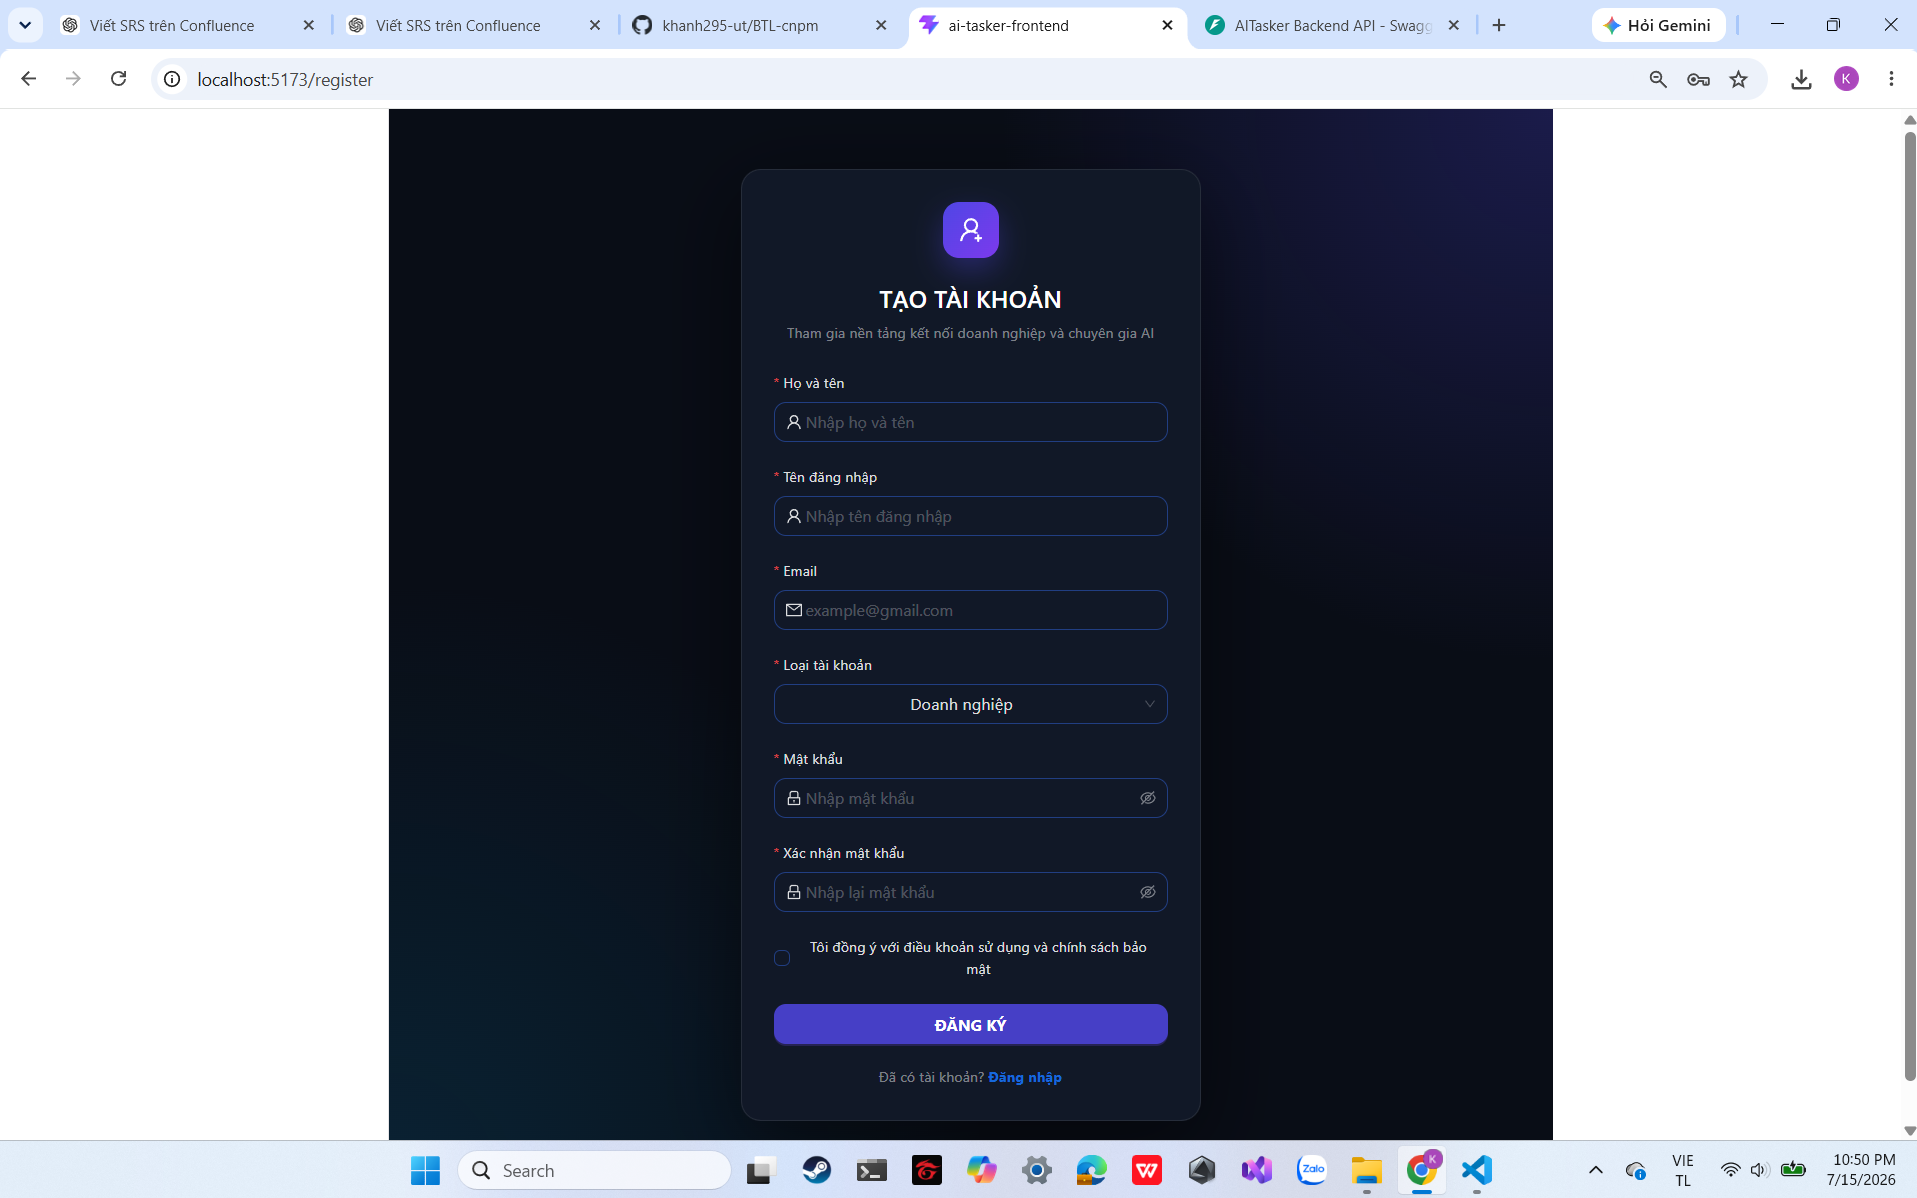
\includegraphics[width=0.78\textwidth]{register.png}
    \caption{Giao diện đăng ký tài khoản AITasker}
    \label{fig:ui-register}
\end{figure}

Thông tin đăng ký gồm:

\begin{itemize}
    \item Họ và tên.
    \item Tên đăng nhập.
    \item Email.
    \item Loại tài khoản.
    \item Mật khẩu và xác nhận mật khẩu.
    \item Xác nhận đồng ý điều khoản sử dụng và chính sách bảo mật.
\end{itemize}

\section{Dashboard tổng quan}
\label{sec:dashboard-interface}

Dashboard hệ thống cung cấp cái nhìn tổng quan về hoạt động của nền tảng. Người quản trị có thể theo dõi tổng số dự án, chuyên gia AI, đề xuất, ngân sách cam kết, lịch sử cập nhật dự án và cơ cấu kỹ năng.

\begin{figure}[H]
    \centering
    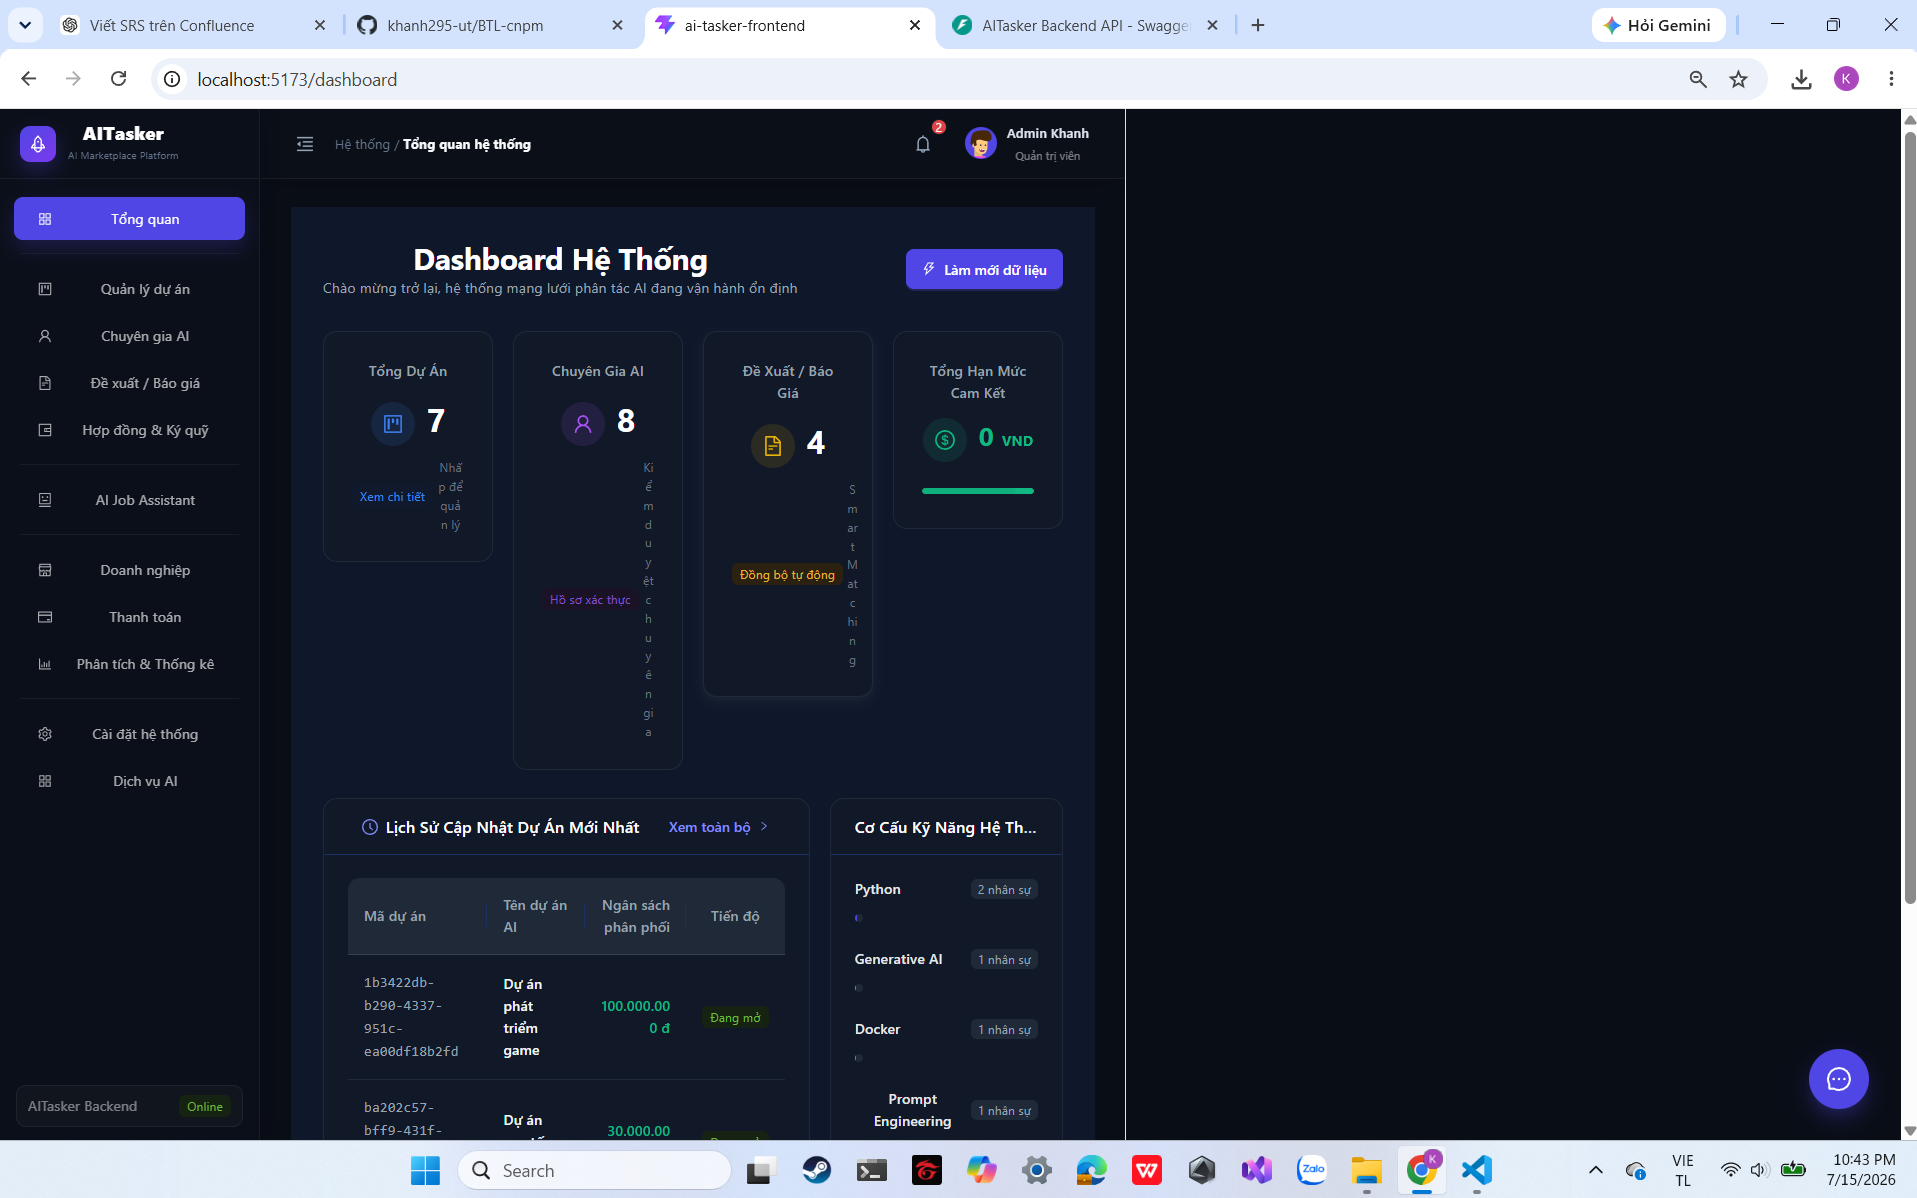
\includegraphics[width=\textwidth]{dashboard.png}
    \caption{Dashboard tổng quan của hệ thống AITasker}
    \label{fig:ui-dashboard}
\end{figure}

Các chỉ số chính được hiển thị gồm:

\begin{itemize}
    \item Tổng số dự án.
    \item Tổng số chuyên gia AI.
    \item Tổng số đề xuất/báo giá.
    \item Tổng hạn mức cam kết.
    \item Các dự án được cập nhật gần nhất.
    \item Cơ cấu kỹ năng AI trong hệ thống.
\end{itemize}

\section{Giao diện quản lý dự án}
\label{sec:project-interface}

Trang quản lý dự án hiển thị danh sách dự án dưới dạng bảng, bao gồm tên dự án, ngân sách, deadline, trạng thái và thao tác. Người dùng có quyền phù hợp có thể tạo mới, cập nhật hoặc xóa dự án.

\begin{figure}[H]
    \centering
    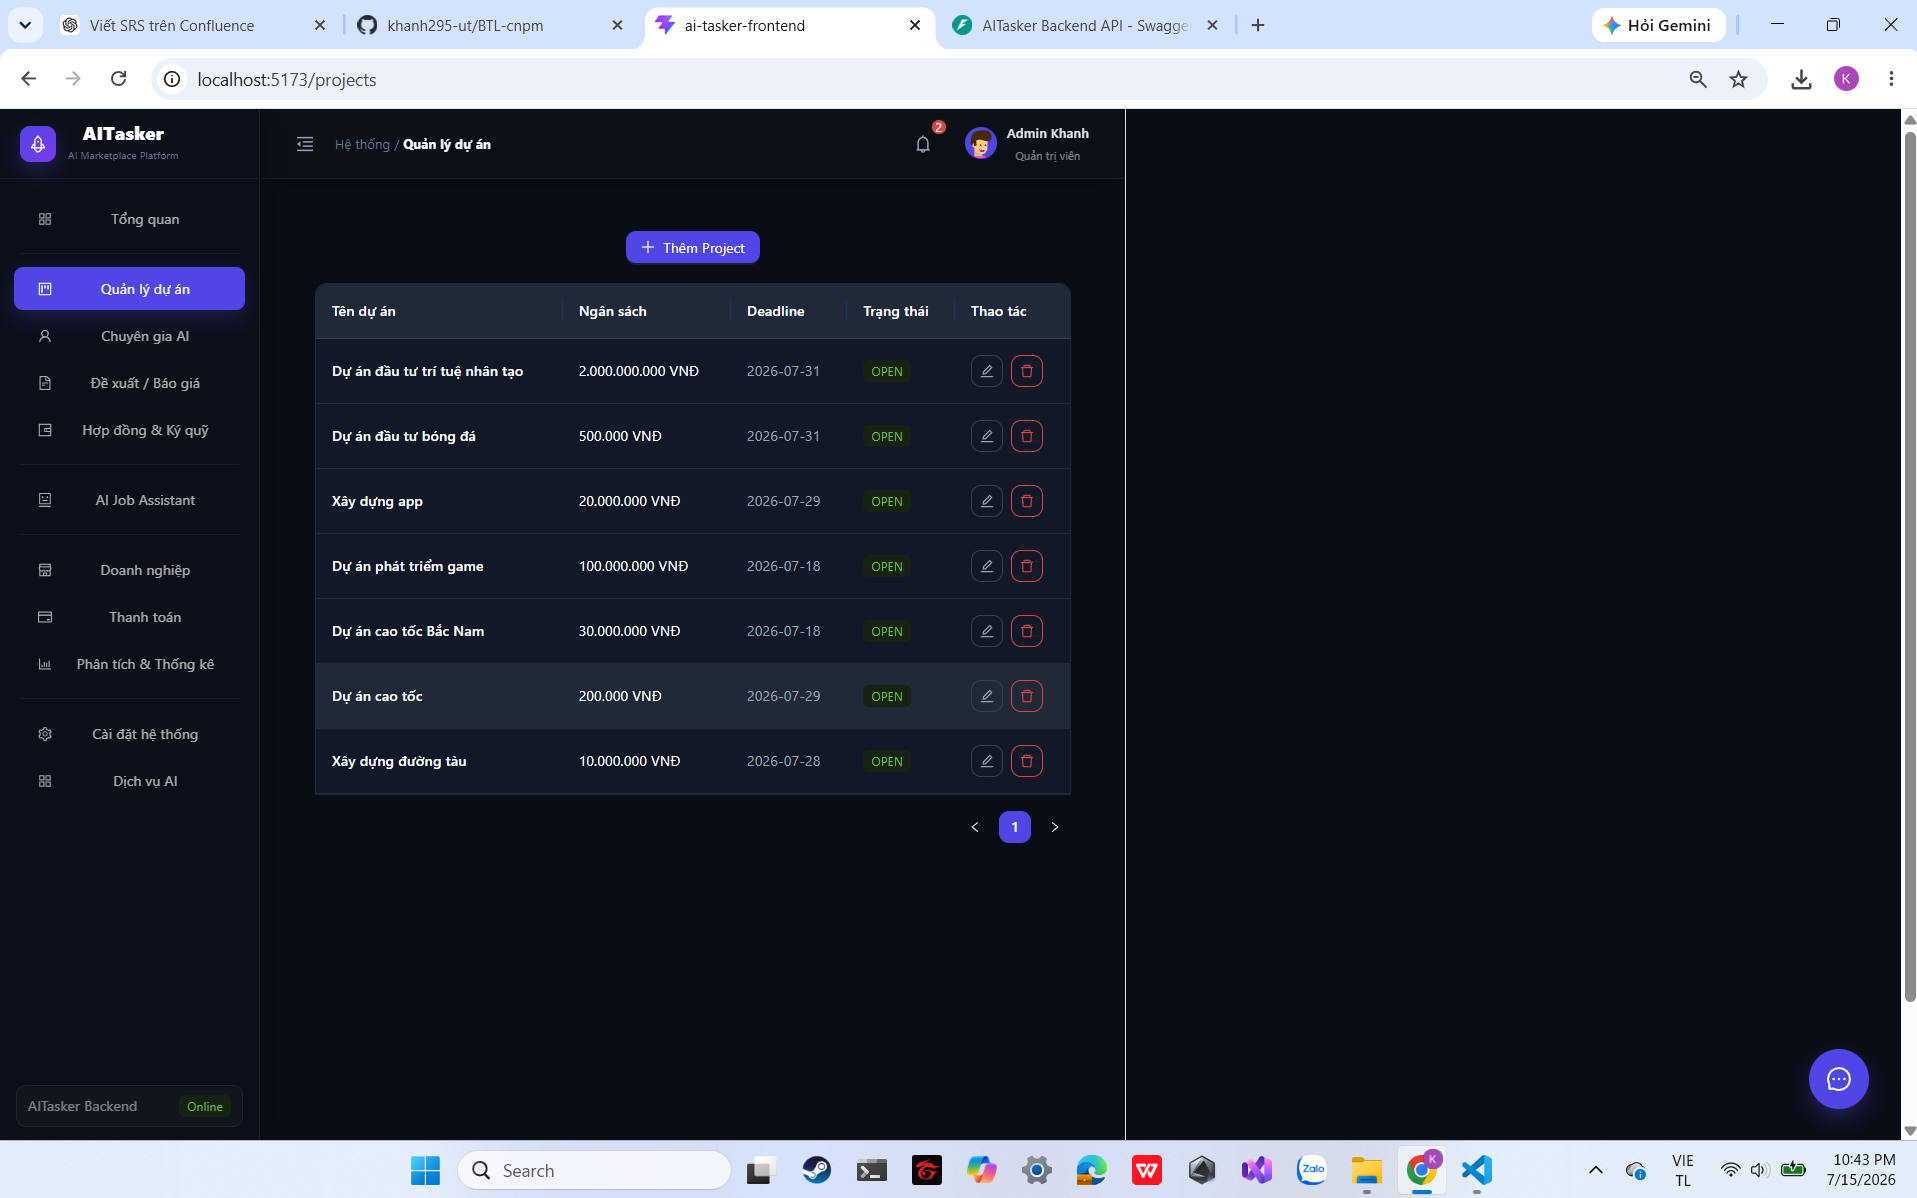
\includegraphics[width=\textwidth]{projects.png}
    \caption{Giao diện quản lý dự án}
    \label{fig:ui-projects}
\end{figure}

Các chức năng chính:

\begin{itemize}
    \item Hiển thị danh sách dự án.
    \item Tạo dự án mới.
    \item Chỉnh sửa dự án.
    \item Xóa hoặc hủy dự án.
    \item Theo dõi trạng thái dự án.
    \item Phân trang danh sách.
\end{itemize}

\section{Giao diện quản lý hợp đồng và ký quỹ}
\label{sec:contract-interface}

Module hợp đồng và ký quỹ hỗ trợ theo dõi giá trị hợp đồng, số tiền đang ký quỹ, số tiền đã giải ngân và danh sách hợp đồng giữa doanh nghiệp với chuyên gia AI.

\begin{figure}[H]
    \centering
    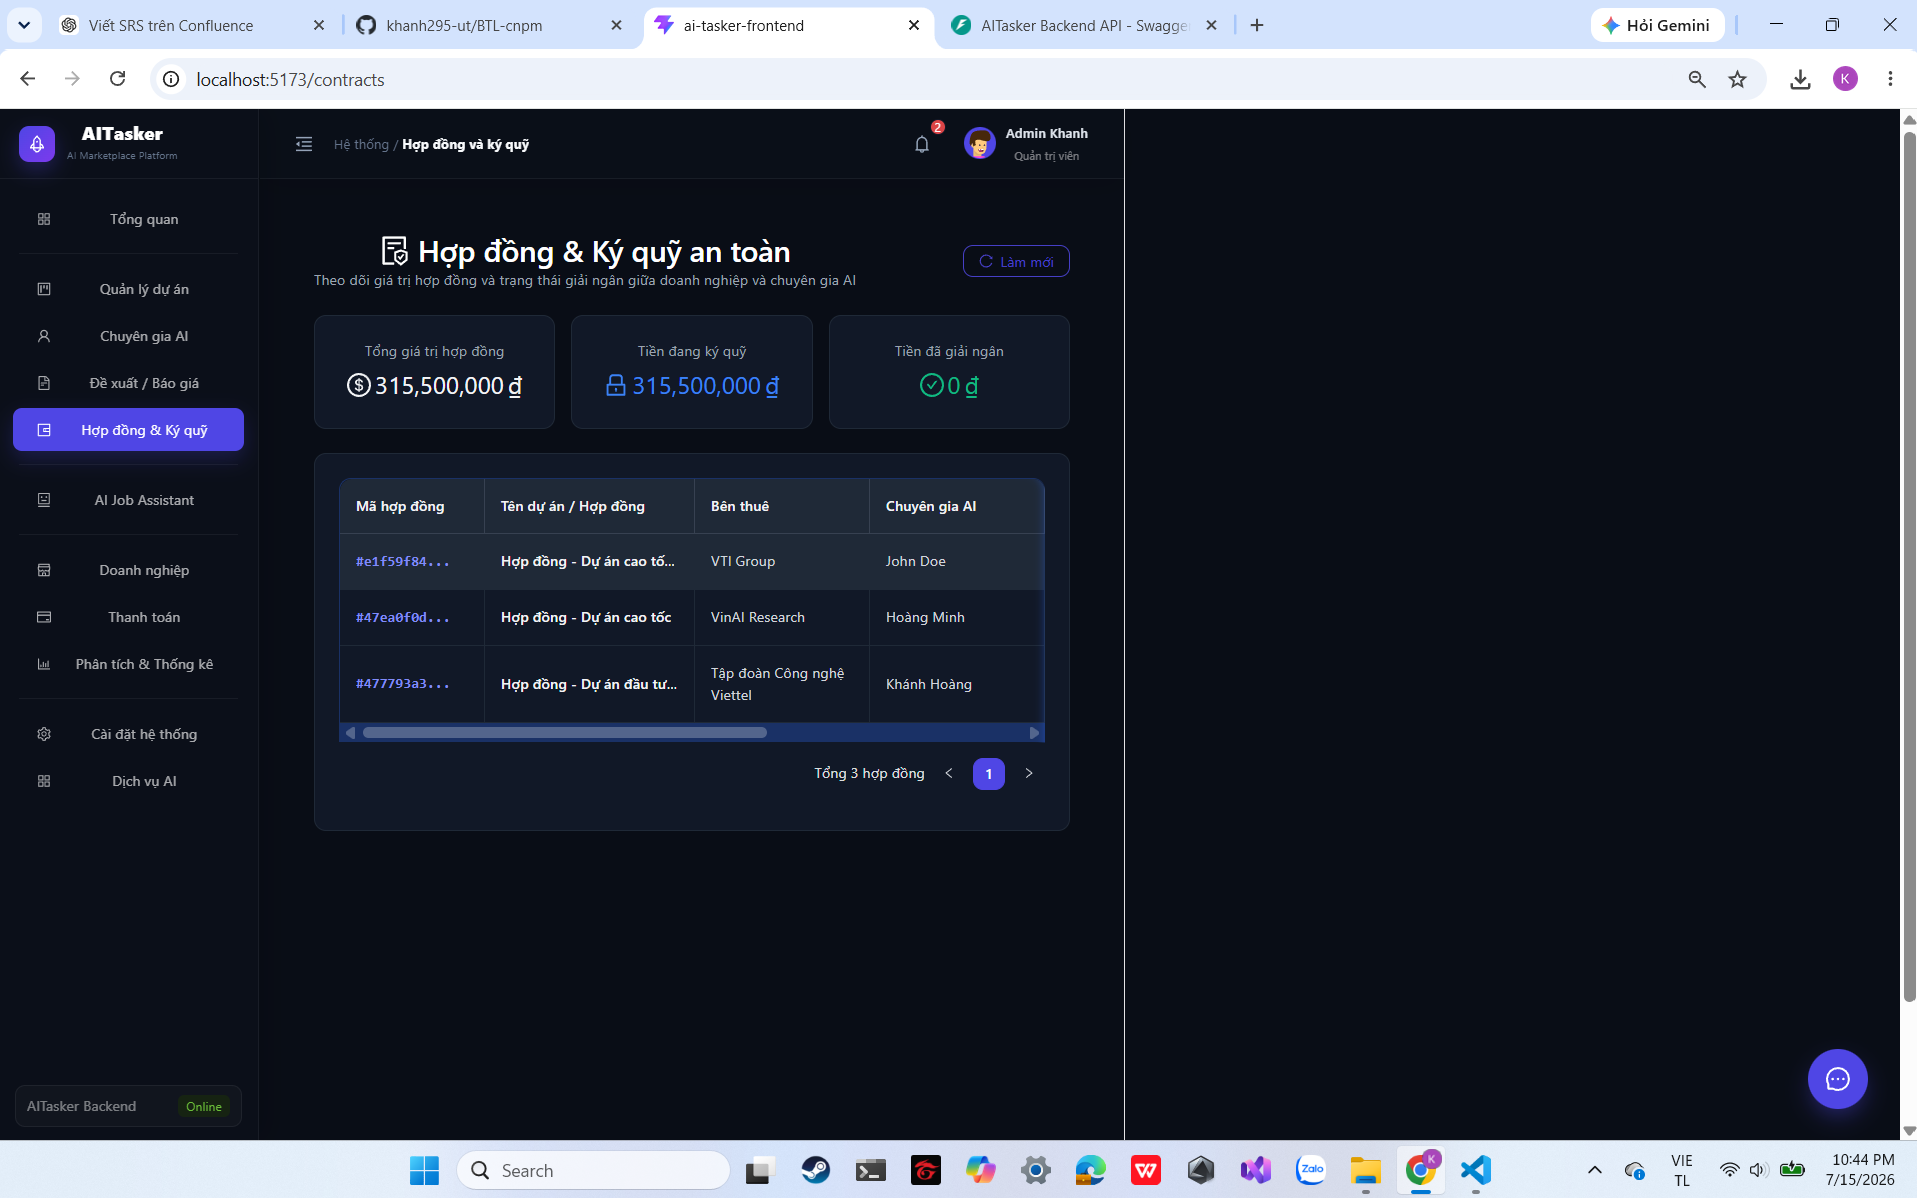
\includegraphics[width=\textwidth]{contracts.png}
    \caption{Giao diện quản lý hợp đồng và ký quỹ}
    \label{fig:ui-contracts}
\end{figure}

Giao diện cho phép:

\begin{itemize}
    \item Theo dõi tổng giá trị hợp đồng.
    \item Theo dõi số tiền đang ký quỹ.
    \item Theo dõi số tiền đã giải ngân.
    \item Xem mã hợp đồng, tên dự án, bên thuê và chuyên gia.
    \item Truy cập chi tiết từng hợp đồng.
\end{itemize}

\section{AI Job Assistant}
\label{sec:ai-assistant-interface}

AI Job Assistant hỗ trợ người dùng chuyển đổi ý tưởng ngắn thành bản mô tả dự án có cấu trúc. Chức năng này sử dụng mô hình Gemini để phân tích ý tưởng và đề xuất danh mục, kỹ năng, ngân sách, thời gian thực hiện, milestone, tiêu chí nghiệm thu và rủi ro.

\begin{figure}[H]
    \centering
    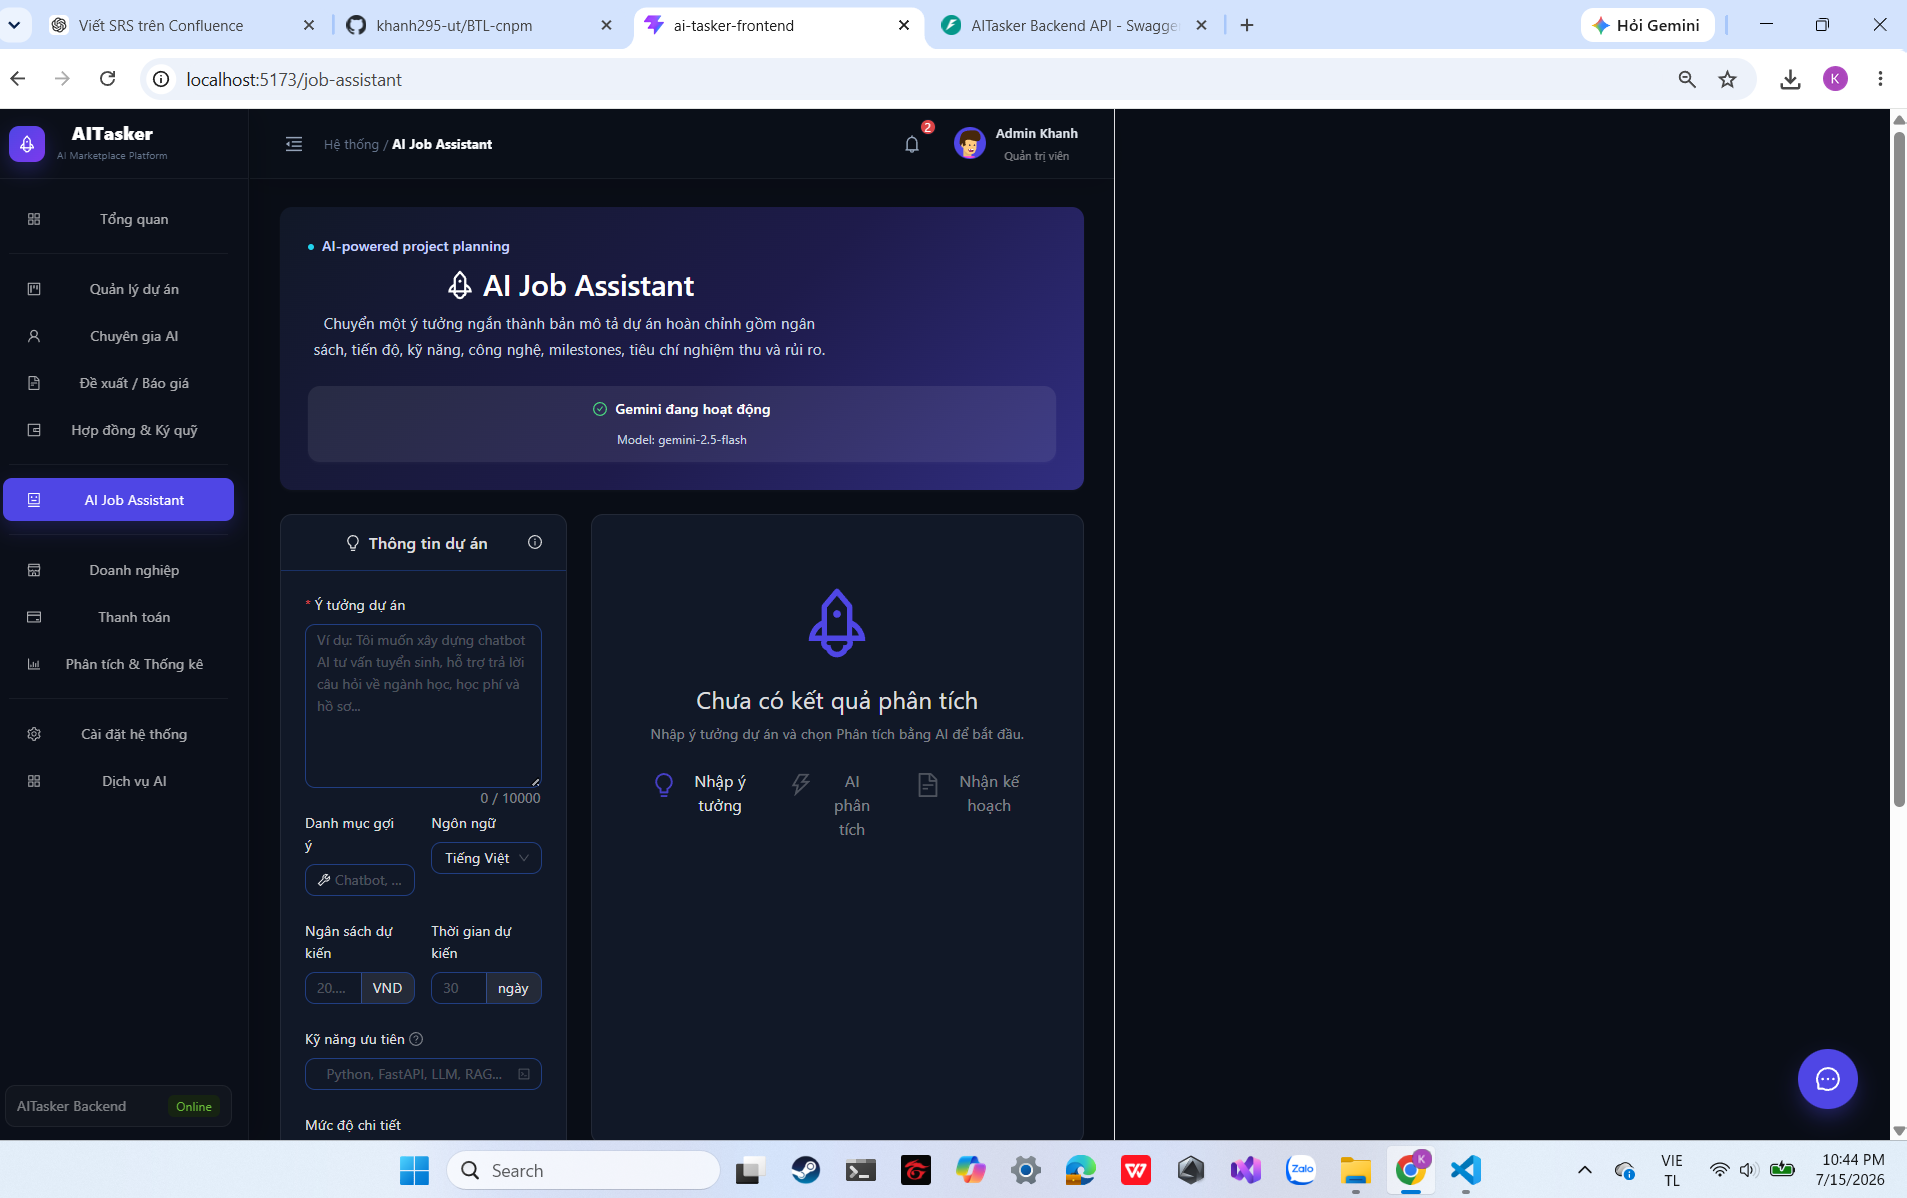
\includegraphics[width=\textwidth]{assistant.png}
    \caption{Giao diện AI Job Assistant}
    \label{fig:ui-ai-assistant}
\end{figure}

Các trường đầu vào gồm:

\begin{itemize}
    \item Ý tưởng dự án.
    \item Danh mục gợi ý.
    \item Ngôn ngữ.
    \item Ngân sách dự kiến.
    \item Thời gian dự kiến.
    \item Kỹ năng ưu tiên.
    \item Mức độ chi tiết.
\end{itemize}

Kết quả phân tích có thể được sử dụng làm dữ liệu khởi tạo cho biểu mẫu tạo dự án.

\section{Giao diện quản lý thanh toán}
\label{sec:payment-interface}

Trang thanh toán lưu trữ và hiển thị lịch sử giao dịch liên quan đến các hợp đồng. Người dùng có thể xem mã giao dịch, số tiền, loại giao dịch, nội dung, thời gian và trạng thái.

\begin{figure}[H]
    \centering
    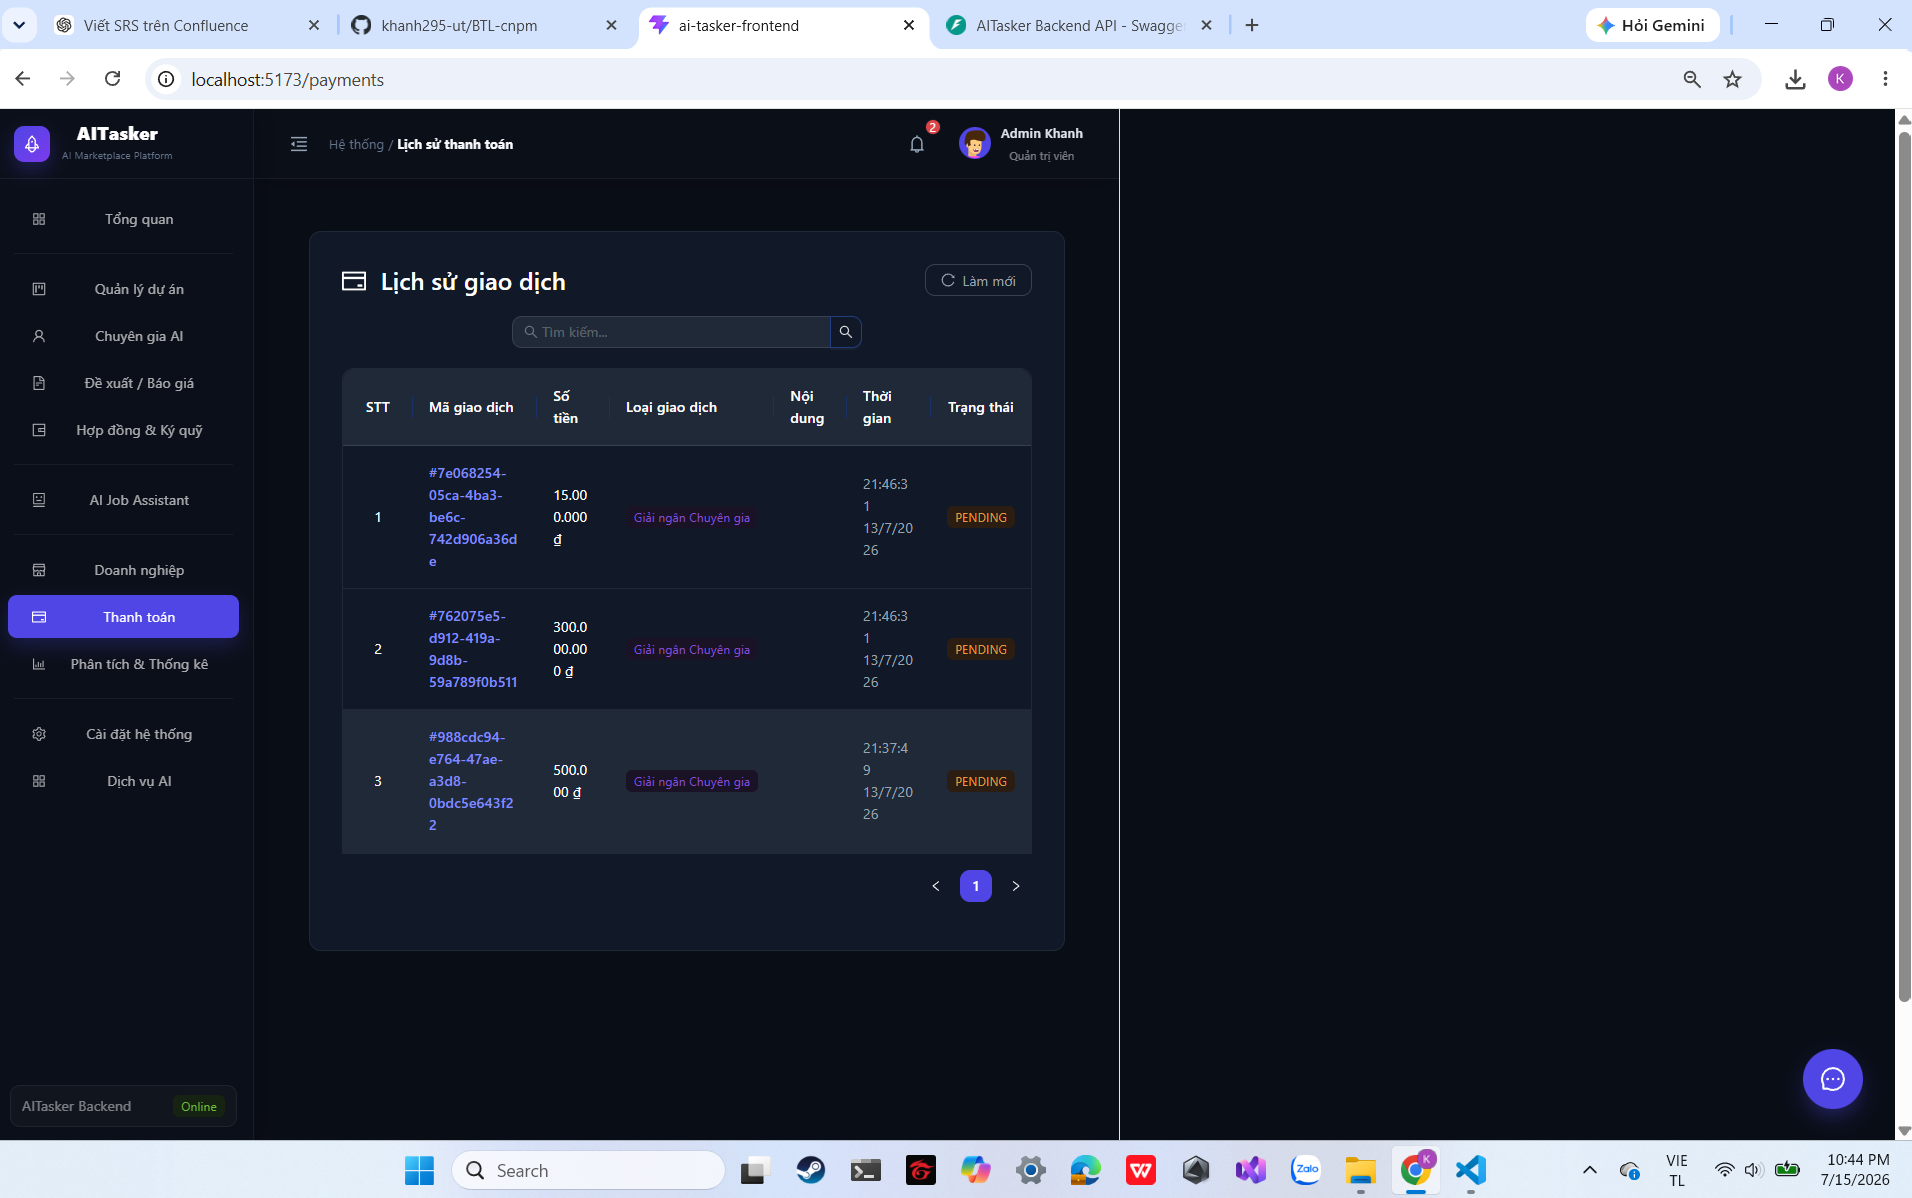
\includegraphics[width=\textwidth]{payment.png}
    \caption{Giao diện lịch sử thanh toán}
    \label{fig:ui-payment}
\end{figure}

Các trạng thái giao dịch có thể gồm:

\begin{itemize}
    \item \texttt{PENDING}
    \item \texttt{PROCESSING}
    \item \texttt{PAID}
    \item \texttt{FAILED}
    \item \texttt{REFUNDED}
\end{itemize}

\section{Giao diện phân tích và thống kê}
\label{sec:analytics-interface}

\subsection{Trung tâm phân tích và báo cáo}

Trang phân tích tổng hợp các chỉ số quan trọng như doanh thu, số chuyên gia hoạt động, số dự án hoàn thành, số dự án đang xử lý, tổng dự án, tổng đề xuất, tổng hợp đồng và giá trị hợp đồng.

\begin{figure}[H]
    \centering
    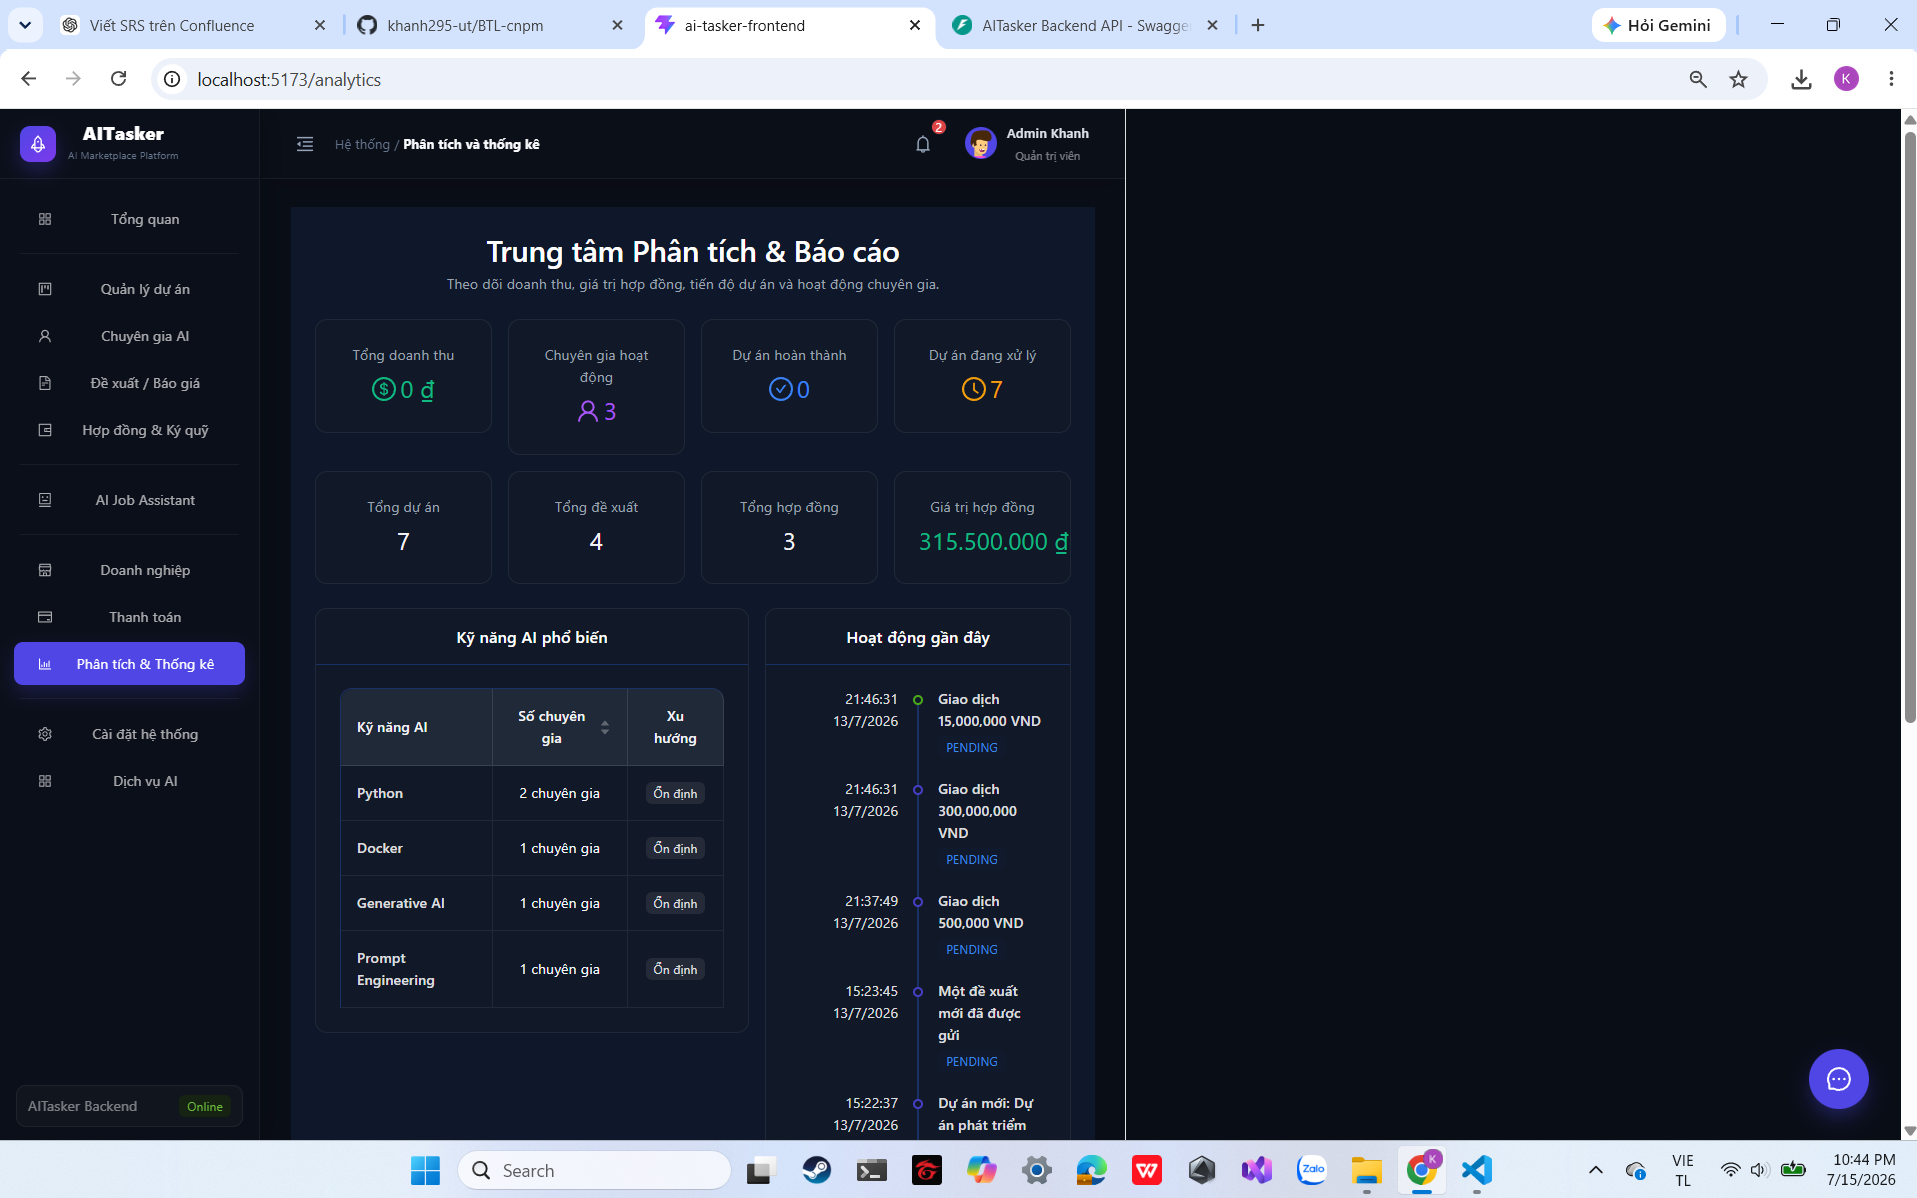
\includegraphics[width=\textwidth]{analytics.png}
    \caption{Giao diện trung tâm phân tích và báo cáo}
    \label{fig:ui-analytics}
\end{figure}

Ngoài các chỉ số tổng hợp, giao diện còn hiển thị kỹ năng AI phổ biến và lịch sử hoạt động gần đây.

\subsection{Dashboard thống kê}

Hệ thống còn cung cấp dashboard thống kê riêng để phục vụ việc theo dõi và đánh giá xu hướng hoạt động theo thời gian.

\begin{figure}[H]
    \centering
    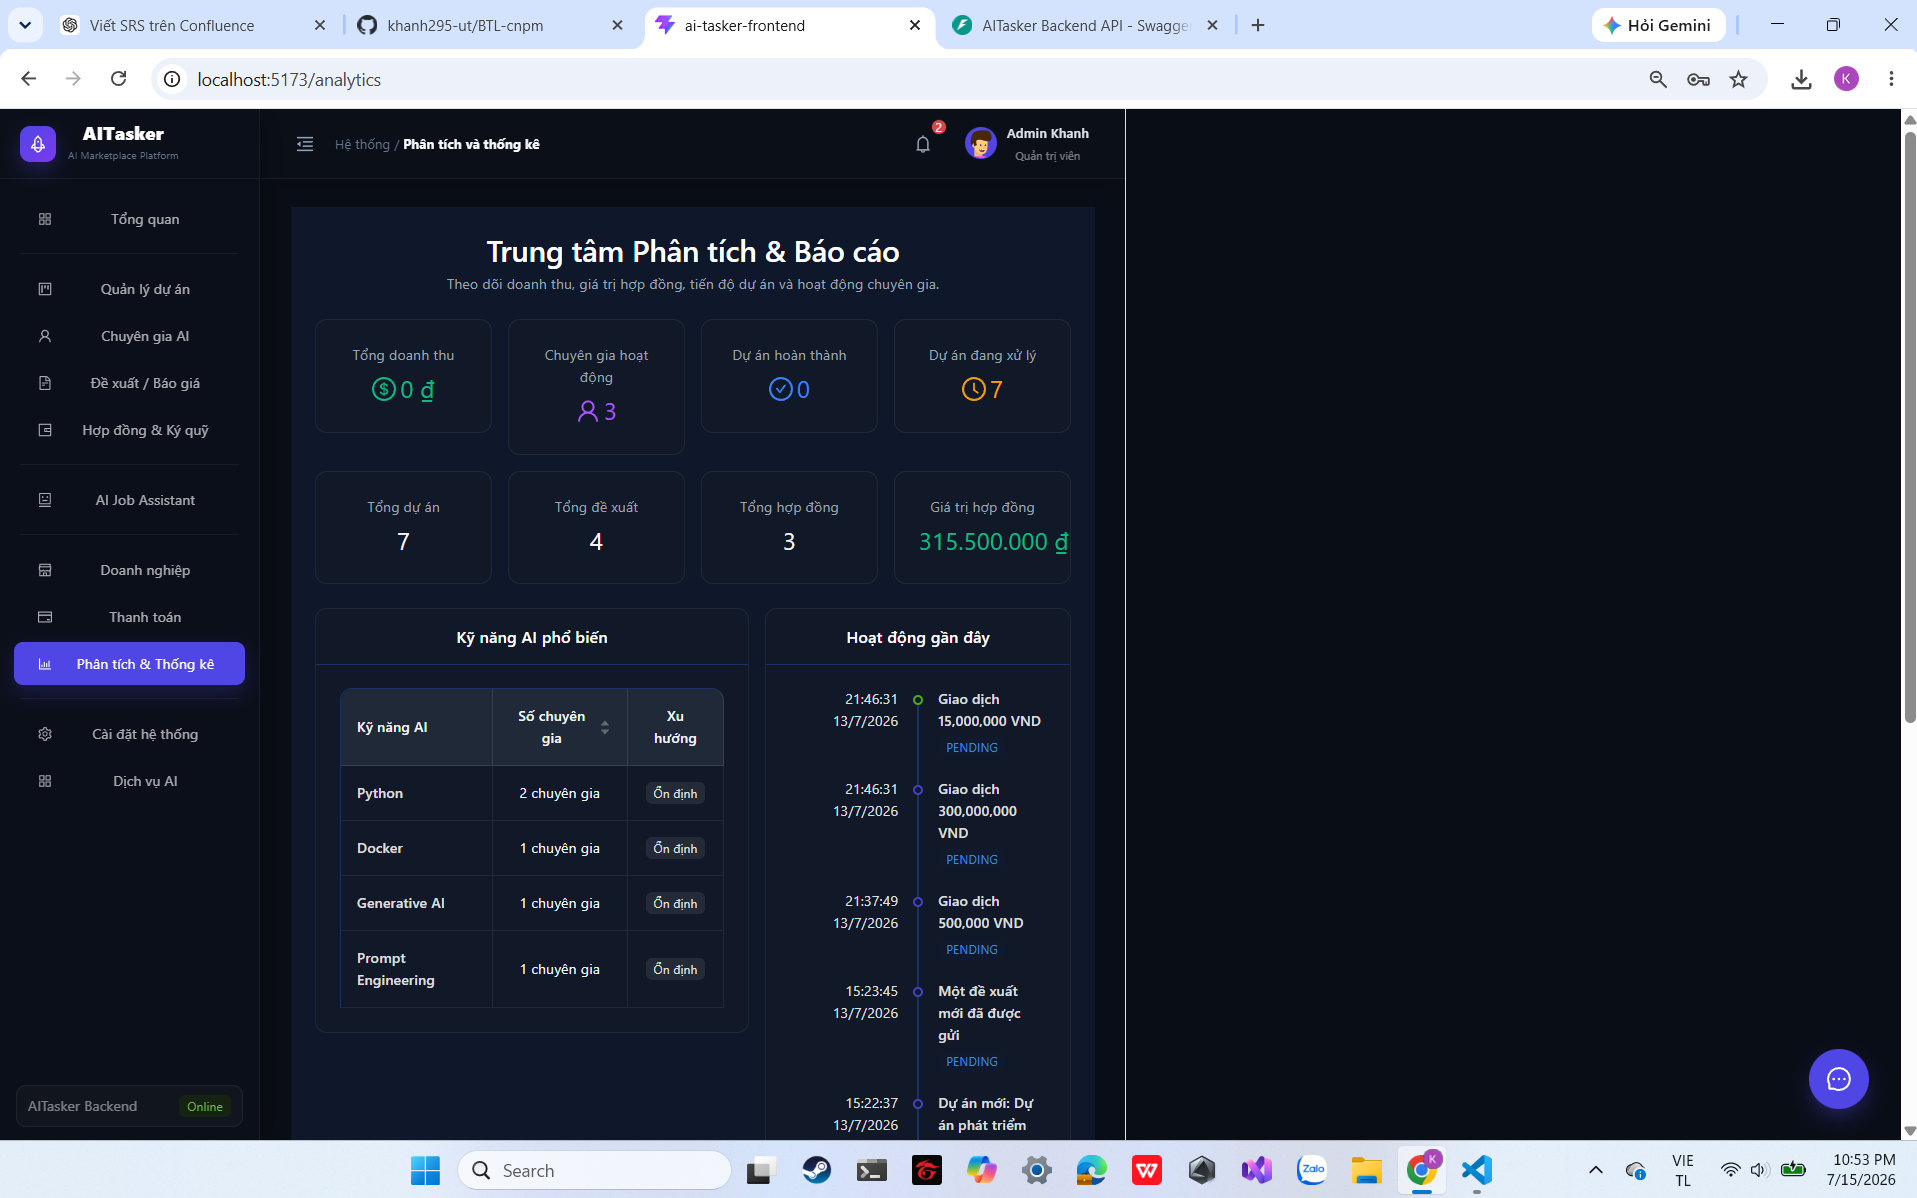
\includegraphics[width=\textwidth]{statistics_dashboard.png}
    \caption{Dashboard thống kê hệ thống}
    \label{fig:ui-statistics-dashboard}
\end{figure}

Việc tách giao diện phân tích và dashboard thống kê giúp hệ thống hỗ trợ cả nhu cầu quan sát nhanh và nhu cầu báo cáo chi tiết.

\section{Marketplace dịch vụ AI}
\label{sec:ai-services-interface}

Marketplace dịch vụ AI cho phép người dùng tìm kiếm các dịch vụ theo từ khóa, danh mục, kỹ năng, mức giá, thời gian thực hiện và loại dịch vụ.

\begin{figure}[H]
    \centering
    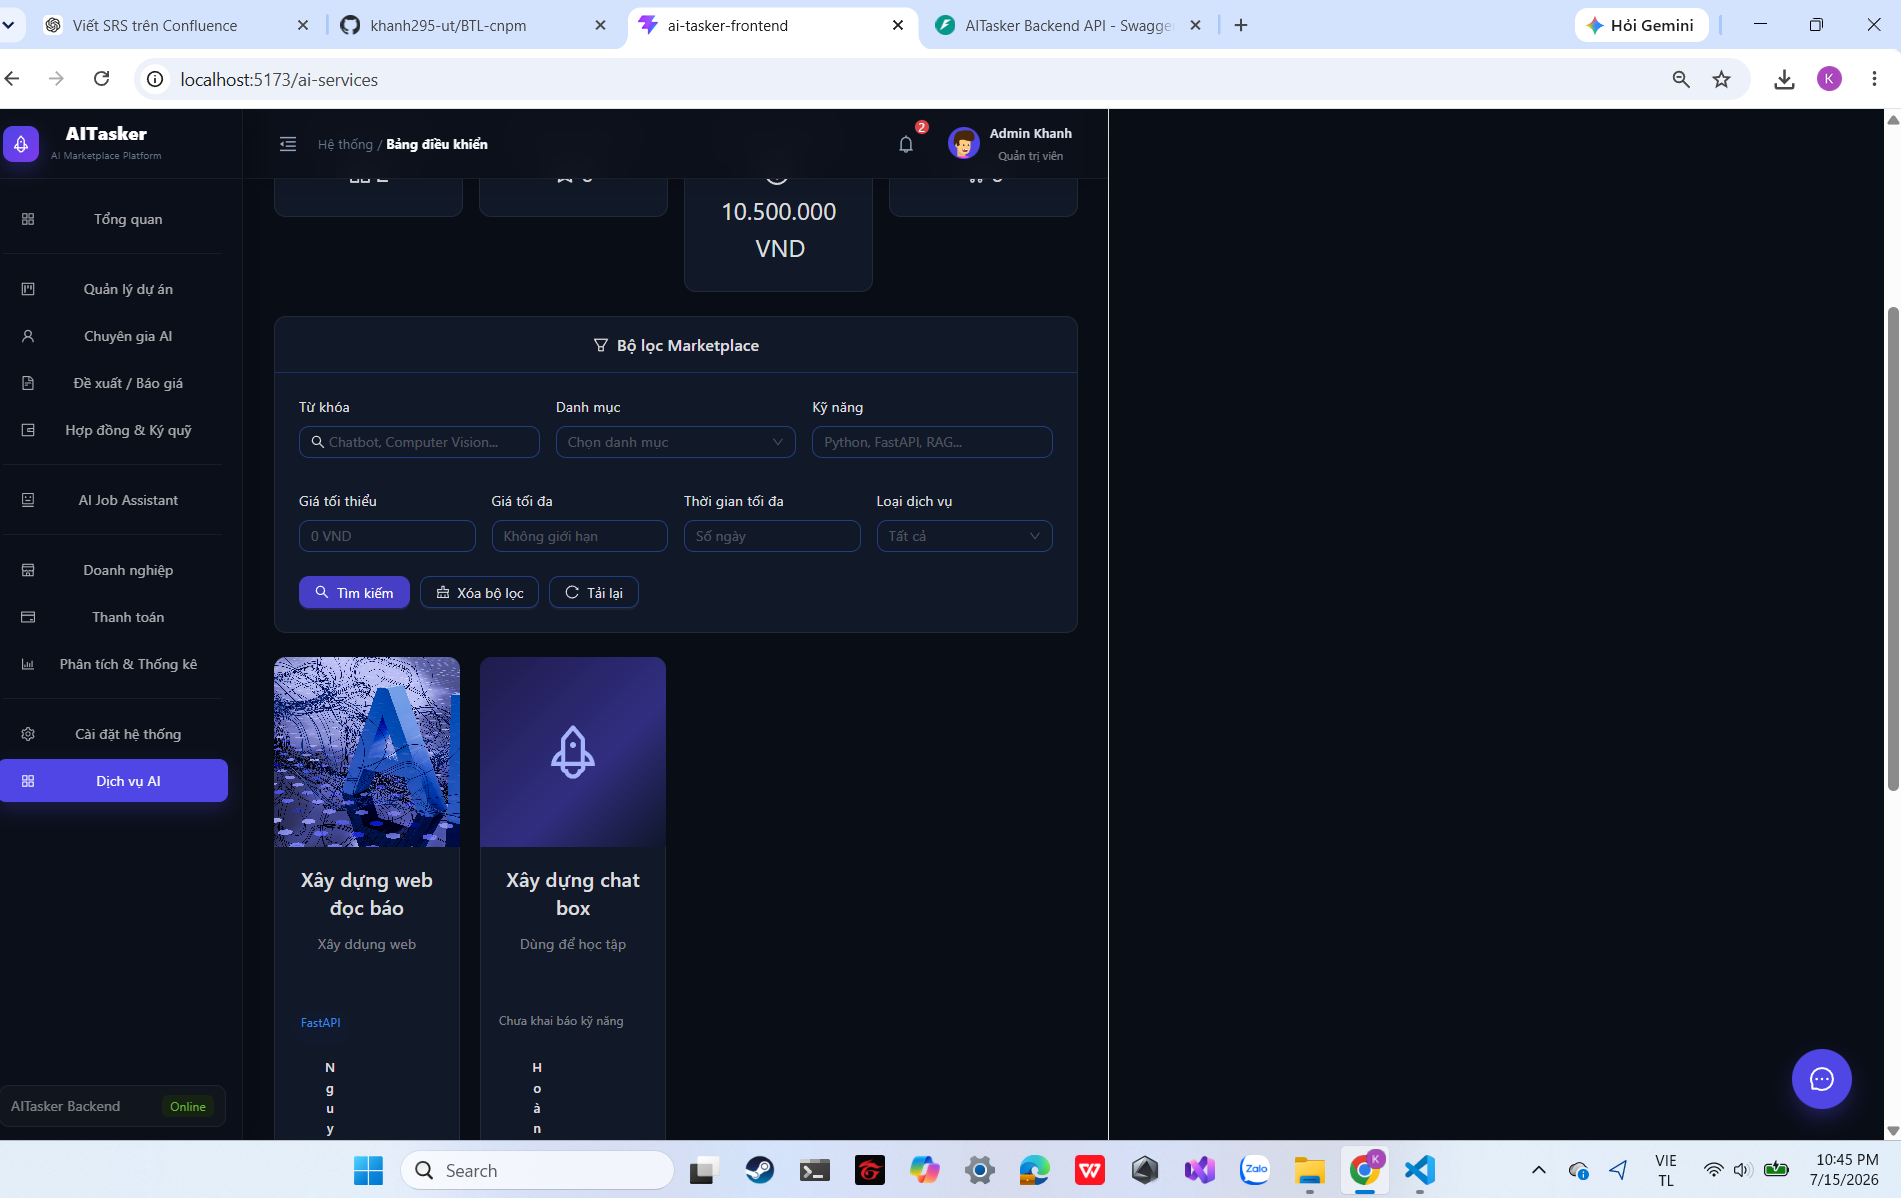
\includegraphics[width=\textwidth]{aiservices.png}
    \caption{Giao diện Marketplace dịch vụ AI}
    \label{fig:ui-ai-services}
\end{figure}

Các chức năng chính:

\begin{itemize}
    \item Tìm kiếm theo từ khóa.
    \item Lọc theo danh mục.
    \item Lọc theo kỹ năng.
    \item Lọc theo mức giá tối thiểu và tối đa.
    \item Lọc theo thời gian hoàn thành.
    \item Hiển thị dịch vụ theo dạng thẻ.
\end{itemize}

\section{Đánh giá tính nhất quán giao diện}
\label{sec:ui-consistency}

Các giao diện của AITasker sử dụng phong cách thiết kế thống nhất:

\begin{itemize}
    \item Tông màu nền tối kết hợp màu tím làm màu nhấn.
    \item Sidebar dùng chung cho các trang quản trị.
    \item Breadcrumb hiển thị vị trí hiện tại.
    \item Các bảng dữ liệu sử dụng định dạng nhất quán.
    \item Trạng thái được biểu diễn bằng nhãn màu.
    \item Các nút thao tác có icon và màu sắc dễ nhận biết.
    \item Thông báo trạng thái backend được hiển thị ở sidebar.
\end{itemize}

Tuy nhiên, một số màn hình còn khoảng trống lớn ở phía bên phải do khu vực nội dung chưa sử dụng toàn bộ chiều rộng. Đây là vấn đề giao diện có thể tiếp tục cải thiện trong phiên bản sau.

\section{Kiểm thử chức năng}
\label{sec:functional-testing-chapter6}

\begin{longtable}{|p{1.5cm}|p{3.4cm}|p{4.0cm}|p{4.0cm}|p{1.3cm}|}
\caption{Các test case chức năng chính}
\label{tab:chapter6-functional-tests} \\ \hline
\textbf{ID} & \textbf{Chức năng} & \textbf{Bước kiểm thử} & \textbf{Kết quả mong đợi} & \textbf{KQ} \\ \hline
\endfirsthead
\hline
\textbf{ID} & \textbf{Chức năng} & \textbf{Bước kiểm thử} & \textbf{Kết quả mong đợi} & \textbf{KQ} \\ \hline
\endhead

TC-01 & Đăng nhập hợp lệ & Nhập đúng email/tài khoản và mật khẩu & Chuyển đến dashboard, nhận JWT hợp lệ & PASS \\ \hline
TC-02 & Đăng nhập sai mật khẩu & Nhập đúng email nhưng sai mật khẩu & Hiển thị thông báo lỗi, không cấp token & PASS \\ \hline
TC-03 & Đăng ký tài khoản & Nhập đầy đủ thông tin hợp lệ & Tạo tài khoản và hồ sơ tương ứng & PASS \\ \hline
TC-04 & Email đăng ký trùng & Đăng ký bằng email đã tồn tại & Từ chối tạo tài khoản & PASS \\ \hline
TC-05 & Xem dashboard & Đăng nhập bằng tài khoản hợp lệ & Hiển thị đúng các chỉ số tổng hợp & PASS \\ \hline
TC-06 & Tạo dự án & Nhập dữ liệu dự án hợp lệ & Tạo Project trạng thái OPEN & PASS \\ \hline
TC-07 & Cập nhật dự án & Chọn dự án thuộc quyền sở hữu và chỉnh sửa & Dữ liệu được cập nhật & PASS \\ \hline
TC-08 & Xem hợp đồng & Truy cập trang hợp đồng & Hiển thị danh sách và số liệu ký quỹ & PASS \\ \hline
TC-09 & AI Job Assistant & Nhập ý tưởng và gửi yêu cầu phân tích & Trả về bản phân tích dự án có cấu trúc & PASS \\ \hline
TC-10 & Xem thanh toán & Truy cập trang lịch sử thanh toán & Hiển thị đúng các giao dịch & PASS \\ \hline
TC-11 & Xem thống kê & Truy cập trang phân tích & Hiển thị đúng chỉ số và dữ liệu gần đây & PASS \\ \hline
TC-12 & Tìm dịch vụ AI & Nhập từ khóa và bộ lọc & Hiển thị danh sách dịch vụ phù hợp & PASS \\ \hline
\end{longtable}

\section{Kiểm thử tích hợp}
\label{sec:integration-testing-chapter6}

\begin{longtable}{|p{1.5cm}|p{4.2cm}|p{4.2cm}|p{4.0cm}|}
\caption{Các luồng kiểm thử tích hợp}
\label{tab:chapter6-integration-tests} \\ \hline
\textbf{ID} & \textbf{Luồng} & \textbf{Thành phần tham gia} & \textbf{Kết quả mong đợi} \\ \hline
\endfirsthead
\hline
\textbf{ID} & \textbf{Luồng} & \textbf{Thành phần tham gia} & \textbf{Kết quả mong đợi} \\ \hline
\endhead

IT-01 & Đăng ký và đăng nhập & React, Auth API, User Service, PostgreSQL & Tài khoản được tạo và đăng nhập thành công. \\ \hline
IT-02 & Tạo dự án & React, Project API, Project Service, PostgreSQL & Dự án được lưu và xuất hiện trong danh sách. \\ \hline
IT-03 & Xem hợp đồng & Contract API, Contract Service, PostgreSQL & Danh sách và tổng giá trị hợp đồng chính xác. \\ \hline
IT-04 & AI Job Assistant & React, AI API, Gemini Service & Kết quả phân tích được trả về và hiển thị. \\ \hline
IT-05 & Lịch sử thanh toán & Payment API, Payment Service, PostgreSQL & Giao dịch hiển thị đúng trạng thái và số tiền. \\ \hline
IT-06 & Phân tích thống kê & Statistics API, nhiều service, PostgreSQL & Chỉ số tổng hợp khớp dữ liệu thực tế. \\ \hline
\end{longtable}

\section{Kiểm thử giao diện}
\label{sec:ui-testing-chapter6}

Các tiêu chí kiểm thử giao diện gồm:

\begin{itemize}
    \item Nội dung hiển thị rõ ràng trên trình duyệt desktop.
    \item Điều hướng sidebar hoạt động đúng.
    \item Các trạng thái loading và lỗi được hiển thị.
    \item Các trường bắt buộc có ký hiệu nhận biết.
    \item Form đăng nhập và đăng ký kiểm tra dữ liệu đầu vào.
    \item Bảng dữ liệu hỗ trợ phân trang.
    \item Nút chỉnh sửa, xóa và làm mới hoạt động đúng.
    \item Màu sắc trạng thái dễ phân biệt.
\end{itemize}

\section{Đánh giá kết quả hiện thực}
\label{sec:implementation-evaluation}

Qua các giao diện và kịch bản kiểm thử, hệ thống đã hiện thực được các chức năng quan trọng:

\begin{itemize}
    \item Đăng ký và đăng nhập.
    \item Dashboard tổng quan.
    \item Quản lý dự án.
    \item Quản lý hợp đồng và ký quỹ.
    \item Trợ lý AI hỗ trợ lập kế hoạch dự án.
    \item Quản lý thanh toán.
    \item Phân tích và thống kê.
    \item Marketplace dịch vụ AI.
\end{itemize}

\subsection{Ưu điểm}

\begin{itemize}
    \item Giao diện đồng nhất và hiện đại.
    \item Dữ liệu frontend được kết nối với backend.
    \item Các module nghiệp vụ chính đã có giao diện sử dụng.
    \item Tích hợp chức năng AI tạo giá trị khác biệt cho hệ thống.
    \item Có dashboard và thống kê phục vụ quản trị.
\end{itemize}

\subsection{Hạn chế}

\begin{itemize}
    \item Một số trang chưa tối ưu chiều rộng nội dung.
    \item Một số bảng có cột dài gây xuống dòng nhiều.
    \item Dữ liệu thanh toán đang ở trạng thái mô phỏng hoặc chờ xử lý.
    \item Chưa có đầy đủ ảnh minh họa cho đề xuất, chuyên gia và doanh nghiệp.
    \item Chưa kiểm thử tải lớn trên môi trường production.
\end{itemize}

\section{Kết luận}
\label{sec:chapter6-conclusion}

Chương này đã trình bày kết quả hiện thực giao diện, các màn hình chức năng chính và quá trình kiểm thử hệ thống AITasker. Các ảnh demo cho thấy hệ thống đã được triển khai ở mức có thể vận hành trên môi trường phát triển, frontend có thể kết nối backend và hiển thị dữ liệu thực tế.

Kết quả đạt được đáp ứng phần lớn yêu cầu chức năng cốt lõi của đồ án. Các vấn đề còn lại chủ yếu liên quan đến tối ưu giao diện, bổ sung dữ liệu thực tế, kiểm thử hiệu năng và hoàn thiện tích hợp dịch vụ bên ngoài.
